% asset_id: AS1QuadraticsTikZ-001
% source: CCEA AS1-AF-LO003, AS1-AF-LO012, AS1-AF-LO014 + quadratics graph sketching evidence
% related_section: Core Theory Part F – Sketching Quadratic Graphs
% purpose: Generic labelled quadratic graph showing roots, y-intercept, turning point and line of symmetry.
\documentclass[tikz,border=8pt]{standalone}
\usetikzlibrary{arrows.meta}
\begin{document}
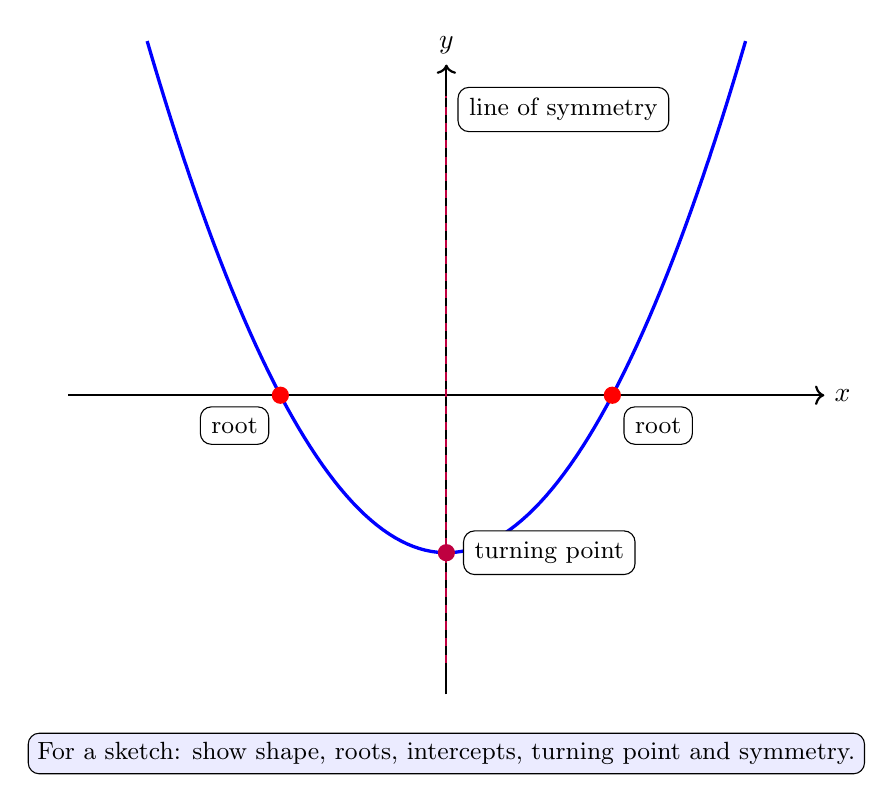
\begin{tikzpicture}[axis/.style={->, thick},curve/.style={very thick, blue},guide/.style={dashed, thick, purple},point/.style={circle, fill=red, inner sep=2.2pt},labelbox/.style={draw, rounded corners, fill=white, inner sep=4pt, font=\small}]
\draw[axis] (-4.8,0) -- (4.8,0) node[right] {$x$};
\draw[axis] (0,-3.8) -- (0,4.2) node[above] {$y$};
\draw[curve, domain=-3.8:3.8, samples=100] plot (\x,{0.45*\x*\x - 2});
\node[point] at (-2.108,0) {}; \node[point] at (2.108,0) {}; \node[point, fill=purple] at (0,-2) {};
\node[labelbox, below left=4pt] at (-2.108,0) {root}; \node[labelbox, below right=4pt] at (2.108,0) {root}; \node[labelbox, right=6pt] at (0,-2) {turning point};
\draw[guide] (0,-3.4) -- (0,3.8); \node[labelbox, above right=4pt] at (0,3.2) {line of symmetry};
\node[draw, rounded corners, fill=blue!8, align=left, font=\small] at (0,-4.55) {For a sketch: show shape, roots, intercepts, turning point and symmetry.};
\end{tikzpicture}
\end{document}
